\subsection{Composer les
plats}\label{diagramme-composer-les-plats}

\begin{figure}
\centering
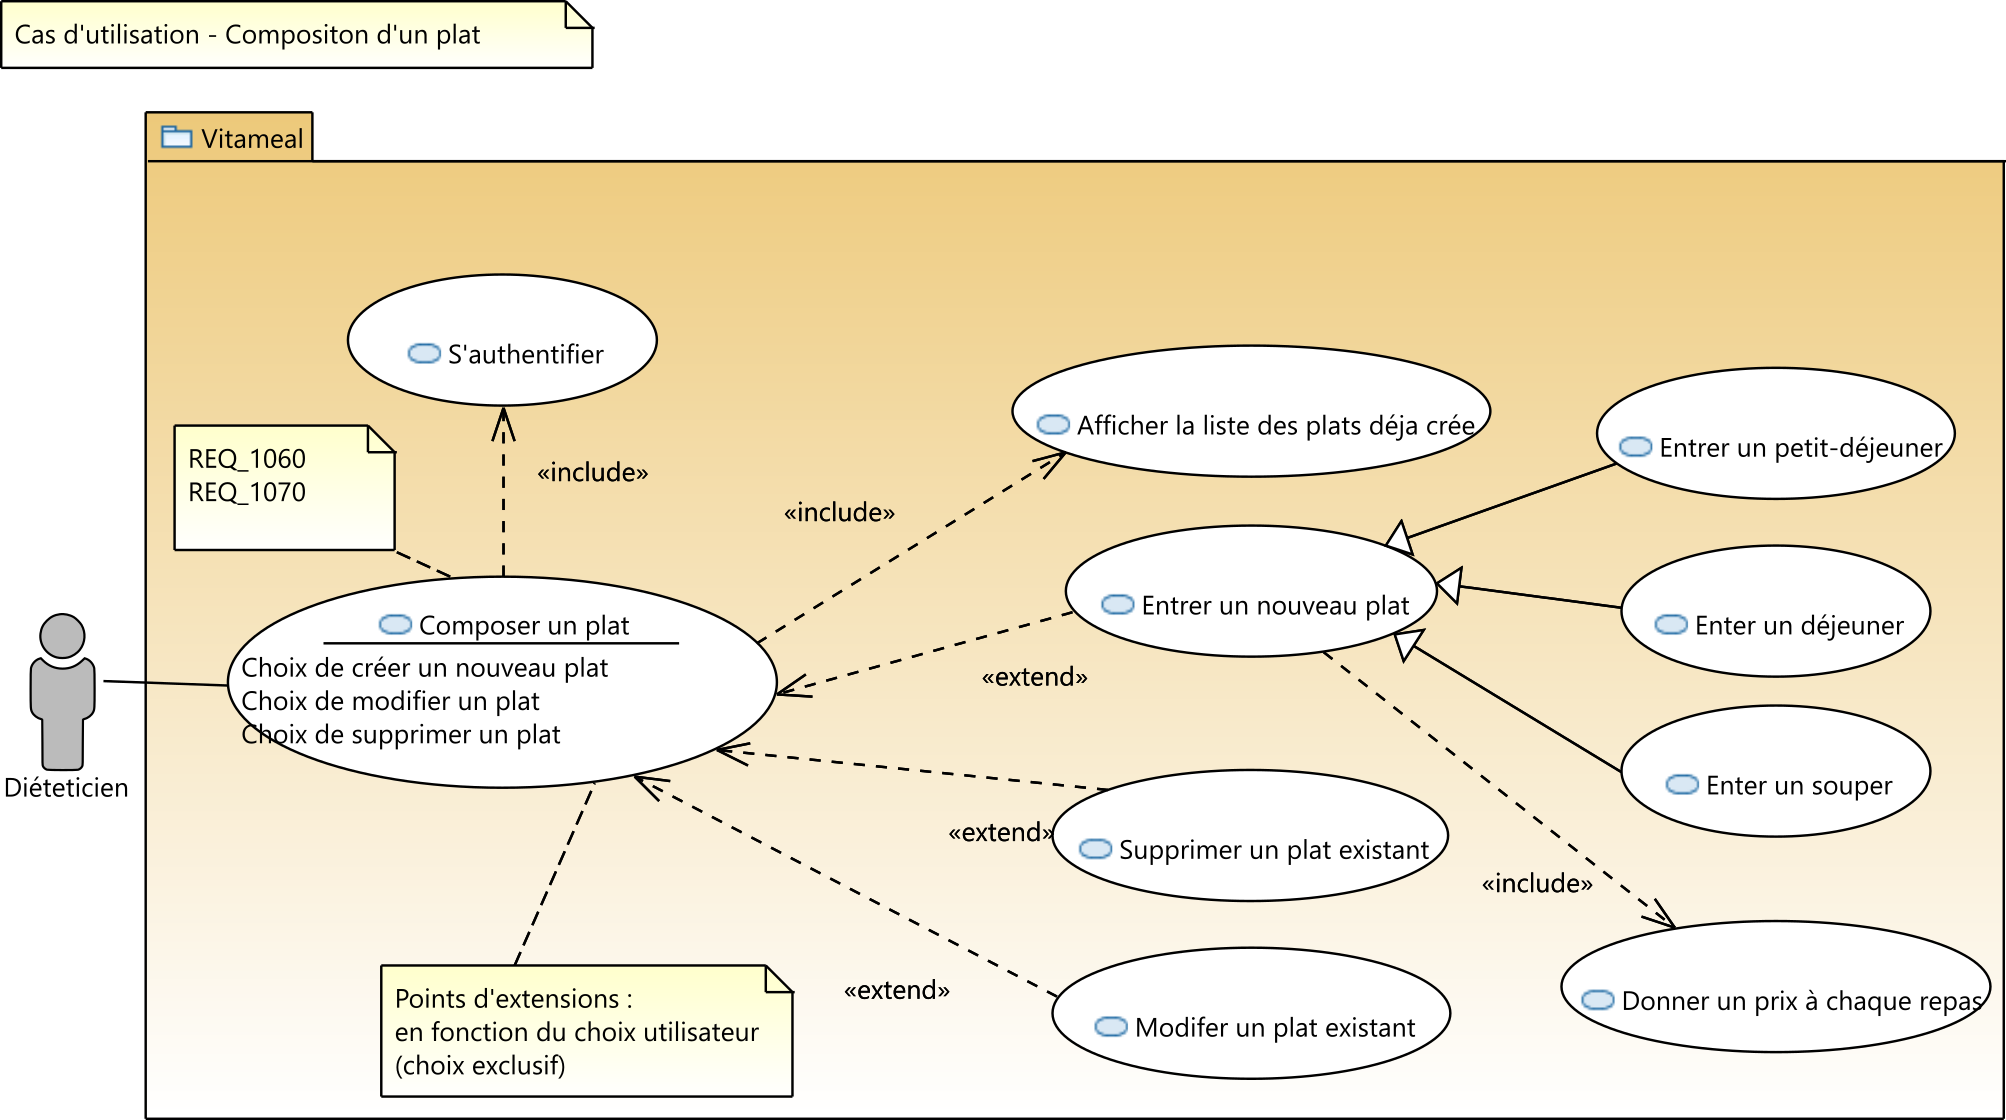
\includegraphics[width=0.9\textwidth]{../../CasDUtilisations/CompositionPlat/uc_composer_un_plat.png}
\caption{Use case composer les plats}
\end{figure}

\subsubsection{UC100 - Composer les
plats}\label{uc100---composer-les-plats}

\noindent\textbf{Nom:} Composer les plats\\
\textbf{ID:} UC100\\
\textbf{Description :} Le diététicien souhaite pouvoir élaborer les
plats composant une journée (petit-déjeuner, déjeuner, souper) en
renseignant leur compositions.\\
\textbf{Auteur :} Nicolas SYMPHORIEN\\
\textbf{Date :} 08/05/2017\\
\textbf{Acteurs :} Le diététicien\\
\textbf{Pré-condition :} L'utilisateur doit être identifié en tant que
diététicien (Voir cas d'utilisation ``S'authentifier'')

\textbf{Scénario principal:}\\
1. Le système affiche la liste des plat déjà créer 2. L'utilisateur
choisi une action :\\
a. L'utilisateur choisi de modifier un plat voir (UC101)\\
b. L'utilisateur choisi de crée un nouveau plat (UC102)\\
c. L'utilisateur choisi de supprimer un plat déjà existant (UC103) 3. Le
système renvoi vers l'écran choisi : ``Modifier un plat'', ``Créer un
plat'' ou affiche une confirmation pour la suppression d'un plat

\textbf{Scénario alternatif:}\\
1. a Le système n'obtient pas la liste des ingrédients

\textbf{Post-Conditions:} L'utilisateur est re-dirigé vers sa sélection.

\subsubsection{UC101 - Modifier un plat
existant}\label{uc101---modifier-un-plat-existant}

\noindent\textbf{Nom:} Modifier un plat existant\\
\textbf{ID:} UC101\\
\textbf{Description :} Le diététicien souhaite pouvoir modifier la
composition d'un plat.\\
\textbf{Auteur :} Nicolas SYMPHORIEN\\
\textbf{Dates :} 08/05/2017\\
\textbf{Acteurs :} Le diététicien\\
\textbf{Pré-condition :} L'utilisateur doit être identifié en tant que
diététicien (Voir cas d'utilisation ``S'authentifier'')

\textbf{Scénario principal :}\\
1. Le système restaure la composition du plat sélectionner et va à
l'étape 3 du cas d'utilisation ``Créer un nouveau plat''

\textbf{Scénario alternatif :}\\
1. a. Le système n'obtient pas la composition du plat sélectionner

\textbf{Post-Conditions:} Le plat est modifié et la modification
enregistrée

\subsubsection{UC102 - Créer un nouveau
plat}\label{uc102---cruxe9er-un-nouveau-plat}

\noindent\textbf{Nom :} Créer un nouveau plat\\
\textbf{ID :} UC102\\
\textbf{Description :} Le diététicien souhaite pouvoir créer la
composition d'un nouveau plat de type petit-déjeuner, déjeuner ou
souper.\\
\textbf{Auteur :} Nicolas SYMPHORIEN\\
\textbf{Dates :} 08/05/2017\\
\textbf{Acteurs :} Le diététicien\\
\textbf{Pré-condition :} L'utilisateur doit être identifié en tant que
diététicien (Voir cas d'utilisation ``S'authentifier'')

\textbf{Scénarios nominal :}\\
1. Le système affiche une page permettant d'entrer la composition d'un
plat 2. L'utilisateur choisi le type de plat (petit-déjeuner, déjeuner,
souper) 3. Le système propose à l'utilisateur une liste de composante à
remplir en fonction du type de plat choisie 4. L'utilisateur choisi les
ingrédients qu'il veut mettre dans chaque composantes 5. L'utilisateur
valide son choix 6. Le système enregistre le nouveau plat dans sa liste
de plats éligible a la composition des menus

\textbf{Scénarios alternatif :}

\begin{enumerate}
\def\labelenumi{\arabic{enumi}.}
\setcounter{enumi}{2}
\item
  \begin{enumerate}
  \def\labelenumii{\alph{enumii}.}
  \item
    L'utilisateur change de type de plat en cours d'élaboration\\
  \end{enumerate}
\item
  \begin{enumerate}
  \def\labelenumii{\alph{enumii}.}
  \setcounter{enumii}{1}
  \item
    Le système propose à l'utilisateur la liste de composante
    correspondante à son nouveau choix (retour etape 3.)\\
  \end{enumerate}
\item
  \begin{enumerate}
  \def\labelenumii{\alph{enumii}.}
  \setcounter{enumii}{2}
  \item
    Le système n'obtient pas la composition du liste des ingrédients\\
  \end{enumerate}
\item
  \begin{enumerate}
  \def\labelenumii{\alph{enumii}.}
  \item
    L'utilisateur annule la composition du plat
  \end{enumerate}
\end{enumerate}

\textbf{Post-Conditions:} Le plat est crée et enregistré

\subsubsection{UC103 - Supprimer un
plat}\label{uc103---supprimer-un-plat}

\noindent\textbf{Nom :} Supprimer un plat\\
\textbf{ID :} UC103\\
\textbf{Description :} Le diététicien souhaite pouvoir supprimer un
plat.\\
\textbf{Auteur :} Nicolas SYMPHORIEN\\
\textbf{Dates :} 08/05/2017\\
\textbf{Acteurs concernés :} Le diététicien\\
\textbf{Pré-condition :} L'utilisateur doit être identifié en tant que
diététicien (Voir cas d'utilisation ``S'autentifier'')

\textbf{Scénarios nominal :}

\begin{enumerate}
\def\labelenumi{\arabic{enumi}.}
\item
  Le système affiche un message d'avertissement avant la suppression
\item
  L'utilisateur confirme ou non la suppression
\item
  Le système supprime le plat de sa liste des plats
\end{enumerate}

\textbf{Scénarios alternatif :}

\begin{enumerate}
\def\labelenumi{\arabic{enumi}.}
\setcounter{enumi}{2}
\item
  \begin{enumerate}
  \def\labelenumii{\alph{enumii}.}
  \item
    Le système ne réussi pas à supprimer le plat
  \end{enumerate}
\end{enumerate}

\textbf{Post-Conditions:} Le plat est supprimé

\subsubsection{UC202 - Donner un prix à chaque
repas}\label{uc202---donner-un-prix-uxe0-chaque-repas}

\noindent\textbf{Nom :} Donner un prix à chaque repas\\
\textbf{ID :} UC202\\
\textbf{Description :} Le service restauration souhaite pouvoir donnée
le pris de chaque plat composant un menu\\
\textbf{Auteur :} Nicolas SYMPHORIEN\\
\textbf{Dates(s) :} 08/05/2017\\
\textbf{Acteurs :} Le service restauration, par héritage, le diététicien
et le médecin\\
\textbf{Pré-condition :} L'utilisateur doit être identifié

\textbf{Scénario principal :}\\
1. Le système propose de renseigner le prix du plat

\textbf{Scénario alternatif :} aucun

\textbf{Post-Conditions:} Le prix du plat est renseigné
